\documentclass[a4paper]{article}
\usepackage[utf8]{inputenc}
\usepackage[spanish, es-tabla]{babel}

\usepackage{amsmath}
\usepackage{amsfonts}
\usepackage{amssymb}

\usepackage{float}
\usepackage{graphicx}
\graphicspath{ {./Imagenes/} }

\usepackage{fancyhdr}

\usepackage{units} 

\pagestyle{fancy}
\fancyhf{}
\lhead{93.54 Métodos Numéricos}
\rhead{Fontecha, Lambertucci, Pouthier, Londero B.}
\rfoot{Página \thepage}



\begin{document}

%%%%%%%%%%%%%%%%%%%%%%%%%%%%%%%%%%%%%%%%%%%%%%%%%%%%%%%%%%%%%%%%%%%%%%%%% 
%								CARATULA								%
%%%%%%%%%%%%%%%%%%%%%%%%%%%%%%%%%%%%%%%%%%%%%%%%%%%%%%%%%%%%%%%%%%%%%%%%% 

\begin{titlepage}
\newcommand{\HRule}{\rule{\linewidth}{0.5mm}}
\center
\mbox{\textsc{\LARGE \bfseries {Instituto Tecnológico de Buenos Aires}}}\\[1.5cm]
\textsc{\Large 93.54 Métodos Numéricos}\\[0.5cm]


\HRule \\[0.6cm]
{ \Huge \bfseries Trabajo práctico N$^{\circ}$2}\\[0.4cm] 
\HRule \\[1.5cm]


{\large

\emph{Grupo 3}\\
\vspace{3px}

\begin{tabular}{lr} 	
\textsc{Fontecha}, María Eugenia  & 58138 \\
\textsc{Lambertucci}, Guido Enrique  & 58009 \\
\textsc{Pouthier}, Florian  & 61337 \\
\textsc{Londero Bonaparte}, Tomás Guillermo  & 58150 \\
\end{tabular}

\vspace{20px}

\emph{Profesor}\\
\vspace{3px}
\textsc{Fierens}, Pablo Ignacio\\ 	
\textsc{Álvarez}, Adrián Omar\\ 

\vspace{100px}

\begin{tabular}{ll}

Presentado: & 02/06/19\\

\end{tabular}

}

\vfill

\end{titlepage}


%%%%%%%%%%%%%%%%%%%%%%%%%%%%%%%%%%%%%%%%%%%%%%%%%%%%%%%%%%%%%%%%%%%%%%%%% 
%								INFORME									%
%%%%%%%%%%%%%%%%%%%%%%%%%%%%%%%%%%%%%%%%%%%%%%%%%%%%%%%%%%%%%%%%%%%%%%%%%


\section{Introducción}
	 \subsection{Sistema de comunicación}
	 	Una forma simple de emular un sistema de comunicación es la presentada a continuación:
	 	\begin{enumerate}
	 		\item	Un emisor transmite un paquete $ s_k $ con un período $ T $, es decir, dicha información es enviada en el instante $ t = nT $, con $ n \in \mathbb{N}_0 $.
	 		\item	La señal es modificada por el canal en la cual se transmite, dependiendo de la respuesta impulsiva del sistema $ {\left \lbrace h_k \right \rbrace}_{k=0}^{L}  $, siendo $ L $ la longitud de la respuesta al impulso.
	 		\item	A lo mencionado anteriormente, se le suma un ruido blanco Gaussiano aditivo $ N_{k}  \sim cN(0,\sigma) $.
 	 	\end{enumerate}
 	 	
 	 	Una vez establecido lo anteriormente mencionado, se pude modelar el sistema de la siguiente forma:
 	 	\begin{equation}
			r_{n} = \sum_{k=0}^{L-1} \; h_{k}s_{n-k} + N_{n}	
 	 	\end{equation}
 	 	
 	 	o también, de la forma matricial:
 	 	\begin{equation}
 	 		\vec{r} = H\vec{s} + \vec{N}
 	 	\end{equation}
 	 	
 	 	con
 	 	\[ \vec{r} =  
 	 		\left( \begin{array}{l}
				r_{0}              \\
				r_{1}              \\
				\vdots 				\\
				r_{n}             
			\end{array} \right)
		,\
 	 	\vec{s} =  
 	 		\left( \begin{array}{l}
				s_{0}              \\
				s_{1}              \\
				\vdots 				\\
				s_{M-1}             
			\end{array} \right)
 	 	,\
 	 	\vec{N} =  
 	 		\left( \begin{array}{l}
				N_{0}              \\
				N_{1}              \\
				\vdots 				\\
				N_{M-1}             
			\end{array} \right)
		,\
 	 	\]
 	 	\par
		\[
		H = 	 	
	 		\left( \begin{array}{lllllllll}
				h_{0}   & 0       & 0       & \hdots  & 0       & 0       & \hdots  & 0       & 0       \\
				h_{1}   & h_{0}   & 0       & \hdots  & 0       & 0       & \hdots  & 0       & 0       \\
				\ddots & \ddots & \ddots & \ddots & 0       & 0       & \hdots  & 0       & 0       \\
				h_{L-1} & h_{L-2} & \hdots   & h_{1}   & h_{0}   & 0	& \hdots  & 0       & 0       \\
				\ddots & \ddots & \ddots & \ddots & \ddots & \ddots & \ddots & \ddots & \ddots \\
				0       & 0       & 0       & 0       & 0       & 0       & \hdots  & h_{1}   & h_{0}  
			\end{array} \right)
		\]
	 	  
		De manera equivalente, se puede escribir la ecuación anterior de la forma:\par
 	 	\begin{equation}
 	 		\vec{r} = S\vec{h} + \vec{N}
 	 		\label{eq:aestimar}
 	 	\end{equation}	\par
 	 	
 	 	con
 	 	\[ \vec{h} =  
 	 		\left( \begin{array}{l}
				h_{0}              \\
				h_{1}              \\
				\vdots 				\\
				h_{L}             
			\end{array} \right)
		,\
		\]
 	 	\[ \vec{S} =
 	 		\left( \begin{array}{lllll}
				s_{0}   & 0       & \hdots      & \hdots	& 0	\\
				s_{1}   & s_{0}   & \hdots      & \hdots	& 0	\\
				\vdots  & \vdots  & \ddots      & \vdots	& \vdots	\\
				s_{L-2} & s_{L-3} & \hdots      & s_{0}	& 0	\\
				s_{L-1} & s_{L-2} & \hdots      & s_{1}	& s_{0}	\\
				s_{L}   & s_{L-1} & \hdots      & s_{2}	& s_{1}	\\
				\vdots	& s_{M-1} & s_{M-2}		& \hdots	& s_{M-L}
			\end{array} \right)
		\]	\par
		
		Finalmente, el objetivo del trabajo es recuperar la señal emitida $ \vec{s} $ partiendo de la recibida  $ \vec{r} $. Generalmente no se conoce ni $ L $ ni $ {\left \lbrace h_k \right \rbrace} $, por lo que estos deben ser estimados.\par
		Si $ L $ es conocido%(para este trabajo se tomará $ L = 5 $)
		, y utilizando la ecuación (\ref{eq:aestimar}) y el método de cuadrados mínimos, se puede encontrar $ \vec{h} \in \mathbb{R}^L $ que minimice
		\begin{equation}
			{\| S\vec{h} - \vec{r} \|}_{2}^{2}
			\label{eq:svd}		
		\end{equation}
		
 	 \subsection{Descomposición en valores singulares}
 	 	El método de descomposición en valores singulares permite resolver ecuaciones de la forma de la ecuación (\ref{eq:svd}), cuando la matriz $ S $ no es de rango completo.
 	 	Este algoritmo busca expresar una matriz $ A \in \mathbb{R}^{m x n}$ (con $ m \geq n $) como el producto de tres matrices:
 	 	\begin{equation}
 	 		A = U \cdot \Sigma \cdot V^{T}
 	 	\end{equation}
 	 	siendo $ U $ y $ V $ matrices ortogonales y $ \Sigma $ una matriz diagonal de valores singulares.\par
 	 	Para poder obtener dicha igualdad, primero se buscan los auto-valores y auto-vectores de $ B = A^{T} \cdot A $. Por un lado, con los auto-valores de $ B $ se obtienen los valores singulares y por consiguiente, la matriz $ \Sigma $, colocandolos en la diagonal de manera decreciente. Por otro lado, $ V $ queda definida como la matriz de  de $ B $.
 	 	Luego se  definen los vectores columna de la matriz $ U $ de la siguiente manera:
 	 	\begin{equation}
 	 		\vec{u}_{i} = A \frac{\vec{v}_{i}}{\sigma_{i}}
		\end{equation} 	 	
 	 	Por convención, los valores singulares se ordenan de foma tal que
 	 	\[ \sigma_{1} \geq \sigma_{2} \geq \ldots \geq \sigma_{r} > \sigma_{r+1} = \sigma_{r+2} = \ldots = \sigma_{n} = 0  \]
 	 	se inventan $ m - r $ vectores más, que sean ortonormales con los anteriores $ \vec{u}_{i} $. Por consiguiente, queda definida la matriz $ U $ como:
 	 	\[ 	U =  
 	 		\left( \begin{array}{llll}
				\vec{u}_{0} & \vec{u}_{1} & \ldots & \vec{u}_{m}
			\end{array} \right)			
		\]
		Retomando el problema planteado para la ecuación (\ref{eq:aestimar}) y utilizando el metodo explicado, se puede dar como solución:
		\begin{equation}
 	 		\vec{h} = \sum_{k=1}^{r} \; \frac{u_{k}^{T} \cdot \vec{r} \cdot v_{k}}{\sigma}
 	 	\end{equation}

\section{Código empleado}
	El código elaborado para este trabajo fue hecho en \textbf{Matlab}.\\
	\begin{itemize}
	\item \textbf{Main:}
		\begin{tabbing}
		function MAIN () L = 5;\\
		ganancia = 0.1;\\
		h = ganancia*(1+randn(L,1));\\
		sigma = 0.1;\\
		a = imread('lena512.bmp');\\
		M = size(a,2);\\
		P = size(a,1);\\
		H = toeplitz([h.' zeros(1,M-L)],zeros(1,M));\\
		r = zeros(M,P);\\
		N = sigma*randn(M,P); \%Noise\\
		s = double(a(:,:)); \\
		r = H*s + N; \% lo que se recibe\\
		b = uint8(r);\\
		figure(1),title('Ejercicio 1,2')\\
		subplot(1,2,1), imshow(a),title('Original') \% 	 la imagen original\\
		subplot(1,2,2), imshow(b),title('Recibida') \% muestro la imagen recibida\\
		E = 512;\\
		sE= zeros(E,1);\\
		for i=1:E\\
		~~~~ sE(i,1) = rand()*256-1;\\
		end\\
		ME= size(sE,1);\\
		PE= size(sE,2);\\
		HE= toeplitz([h.' zeros(1,ME-L)],zeros(1,ME));\\
		rE= zeros(ME,PE);\\
		NE= sigma*randn(ME,PE); \% ruido\\
		\% se transmite\\
		rE = HE*sE + NE; \% lo que se recibe\\
		\% estimo h\\
		S = toeplitz(sE');\\
		S = S(:,1:L);\\
		S = tril(S);\\
		he = estimate(S,rE);\\
		He= toeplitz([he.' zeros(1,M-L)],zeros(1,M));\\
		CN= sigma\^2*eye(size(He)); \% matriz de covarianza del ruido\\
		sigmax= sqrt(1/256*(sum(((0:255)-mean(0:255)).\^2)));\\
		\%dispersión de los símbolos enviados\\
		mx= mean(0:255)*ones(M,1); \% media de los símbolos enviados\\
		CX= sigmax\^2*eye(size(He)); \% matriz de covarianza de los\\
		\%simbolos enviados - asume independencia\\
		W = CX*He'*inv(He*CX*He'+CN); \% matriz de ecualización\\
		d = zeros(M,P);\\
		for k = 1:P\\
		~~~~ d(:,k) = W*(r(:,k)-He*mx)+mx;\\
		end\\
		d = uint8(d);\\
		figure(2),title('Ejercicio 3')\\
		subplot(1,3,1), imshow(a),title('Original')  \% muestro la imagen original\\
		subplot(1,3,2), imshow(b),title('Recibida') \% muestro la imagen recibida\\
		subplot(1,3,3), imshow(d),title('Estimada') \% muestro la imagen estimada
		\end{tabbing}

	\item \textbf{Función ``estimate":}
		\begin{tabbing}		
		function he = estimate (S, rE)\\
		$ [ $U,S,V$ ] $ = DVS(S);\\
		he = zeros(size(V,2),1);\\
		for k=1:size(V,2)\\
		~~~~ he= he+(U(:,k)'*rE*V(:,k))/S(k,k);\\
		end
		\end{tabbing}
		
 	\item \textbf{Función ``DVS":}
 		\begin{tabbing}
		function $ [ $U,S,V$ ] $ = DVS (A)\\
	  	m = size(A,1);\\
		n = size(A,2);\\
		Uprov = zeros(m,m);\\
		V = zeros(n,n);\\	
		S = zeros(m,n);\\
		B=A'*A;\\
		$ [ $V,sigma$ ] $ = eig(B);\\
		sigma2 = sort(diag(sigma),'descend');\\
		V=fliplr(V);\\
		Sig=sqrt(sigma2);\\
		for k = 1:size(Sig)\\
		~~~~ S(k,k)=Sig(k);\\
	 	end\\
		for k=1:n\\
		~~~~ Uprov(:,k)=(A * V(:,k))/Sig(k);\\
		end\\
		if size(Uprov,2) < m\\
		~~~~ U = completar(Uprov);\\
		else\\
		~~~~ U = Uprov;\\
	 	end
		\end{tabbing}
		
	\item \textbf{Función ``completar":}
 		\begin{tabbing}
 		function [Ucompleta] = completar(U)
		\%completar U toma una matriz U de m*n \\
		\%y devuelve otra matriz de m*m ortonormal\\
		$ [ $ m,n $ ] $ = size(U);\\
		U = $ [ $ U zeros(m, m-n) $ ] $;\\
		for i = 1:(m-n)\\
    	~~~~ vec = rand([m 1]);\\
    	~~~~ vecOrt = vec - sum(((vec'*U).*U),2); \%ortogonalización de vec\\
    	~~~~ U(:,n+i) = vecOrt/norm(vecOrt); \%normalización del vector\\
		end\\
		Ucompleta = U;\\
    	end
 		\end{tabbing}	
 	\end{itemize}
	
\section{Resultados obtenidos} 
	A continuación, se presentan los resultados obtenidos de la simulación. Cabe aclarar que, para poder realizar la estimación, se establecieron valores tales como la longitud de la respuesta impulsiva $ L = 5 $ y la ganancia $ h = 0.1 $. Para los parámetros de longitud $ E $ y el desvío estándar $ \sigma $, se repitió el proceso con distintos valores:
\begin{itemize}
	
	\item $ E = 32 $
	\begin{figure}[H]
		\centering
		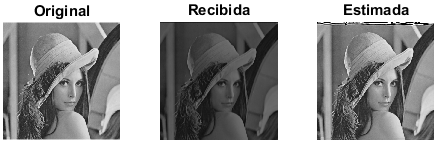
\includegraphics[width=0.9\textwidth]{E32S0.png}
		\caption{Iteración con $ E = 32 $ y $ \sigma = 0 $.}
	\end{figure}	
	\begin{figure}[H]
		\centering
		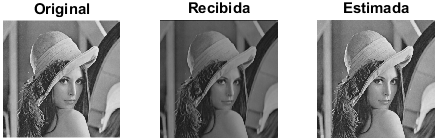
\includegraphics[width=0.9\textwidth]{E32S01.png}
		\caption{Iteración con $ E = 32 $ y $ \sigma = 0.1 $.}
	\end{figure}
	\begin{figure}[H]
		\centering	
		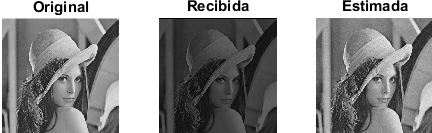
\includegraphics[width=0.9\textwidth]{E32S1.png}
		\caption{Iteración con $ E = 32 $ y $ \sigma = 1 $.}
	\end{figure}		
	\begin{figure}[H]
		\centering		
		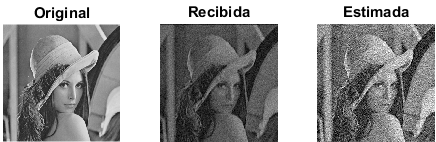
\includegraphics[width=0.9\textwidth]{E32S10.png}
		\caption{Iteración con $ E = 32 $ y $ \sigma = 10 $.}
	\end{figure}		
	\begin{figure}[H]
		\centering		
		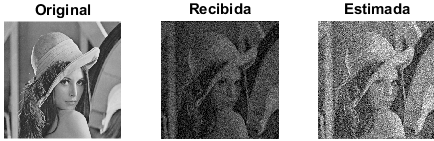
\includegraphics[width=0.9\textwidth]{E32S20.png}
		\caption{Iteración con $ E = 32 $ y $ \sigma = 20 $.}
	\end{figure}		
	\begin{figure}[H]
		\centering	
		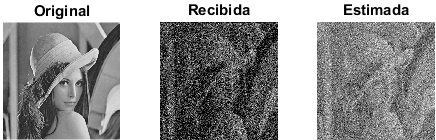
\includegraphics[width=0.9\textwidth]{E32S50.png}
		\caption{Iteración con $ E = 32 $ y $ \sigma = 50 $.}
	\end{figure}		
	\begin{figure}[H]
		\centering		
		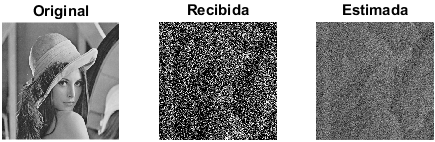
\includegraphics[width=0.9\textwidth]{E32S100.png}
		\caption{Iteración con $ E = 32 $ y $ \sigma = 100 $.}
	\end{figure}
	
	\pagebreak
	\item $ E = 512 $
	\begin{figure}[H]
		\centering
		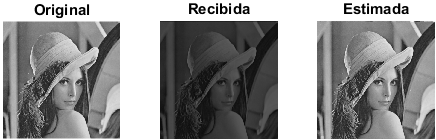
\includegraphics[width=0.9\textwidth]{E512S0.png}
		\caption{Iteración con $ E = 512 $ y $ \sigma = 0 $.}
	\end{figure}	
	\begin{figure}[H]
		\centering
		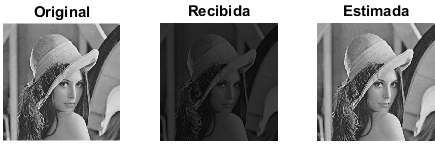
\includegraphics[width=0.9\textwidth]{E512S01.png}
		\caption{Iteración con $ E = 512 $ y $ \sigma = 0.1 $.}
	\end{figure}
	\begin{figure}[H]
		\centering	
		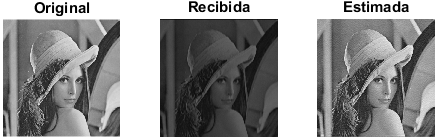
\includegraphics[width=0.9\textwidth]{E512S1.png}
		\caption{Iteración con $ E = 512 $ y $ \sigma = 1 $.}
	\end{figure}		
	\begin{figure}[H]
		\centering		
		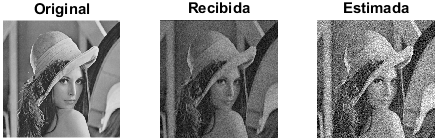
\includegraphics[width=0.9\textwidth]{E512S10.png}
		\caption{Iteración con $ E = 512 $ y $ \sigma = 10 $.}
	\end{figure}		
	\begin{figure}[H]
		\centering		
		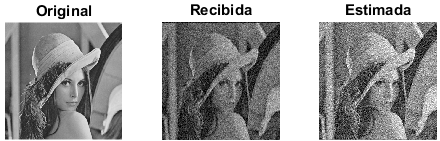
\includegraphics[width=0.9\textwidth]{E512S20.png}
		\caption{Iteración con $ E = 512 $ y $ \sigma = 20 $.}
	\end{figure}		
	\begin{figure}[H]
		\centering	
		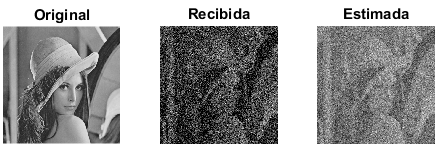
\includegraphics[width=0.9\textwidth]{E512S50.png}
		\caption{Iteración con $ E = 512 $ y $ \sigma = 50 $.}
	\end{figure}		
	\begin{figure}[H]
		\centering		
		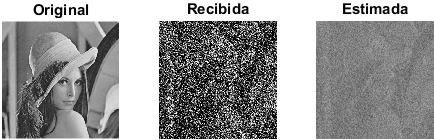
\includegraphics[width=0.9\textwidth]{E512S100.png}
		\caption{Iteración con $ E = 512 $ y $ \sigma = 100 $.}
	\end{figure}
	
	\pagebreak
	\item $ E = 1024 $
	\begin{figure}[H]
		\centering
		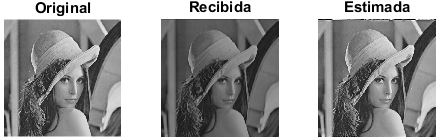
\includegraphics[width=0.9\textwidth]{E1024S0.png}
		\caption{Iteración con $ E = 1024 $ y $ \sigma = 0 $.}
	\end{figure}
	\begin{figure}[H]
		\centering
		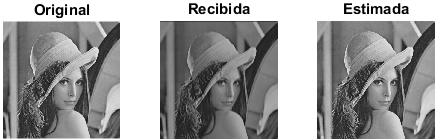
\includegraphics[width=0.9\textwidth]{E1024S01.png}
		\caption{Iteración con $ E = 1024 $ y $ \sigma = 0.1 $.}
	\end{figure}
	\begin{figure}[H]
		\centering
		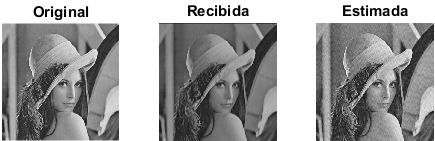
\includegraphics[width=0.9\textwidth]{E1024S1.png}
		\caption{Iteración con $ E = 1024 $ y $ \sigma = 1 $.}
	\end{figure}
	\begin{figure}[H]
		\centering
		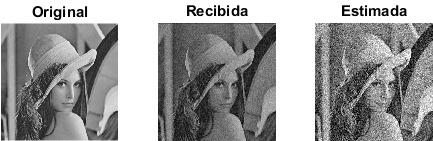
\includegraphics[width=0.9\textwidth]{E1024S10.png}
		\caption{Iteración con $ E = 1024 $ y $ \sigma = 10 $.}
	\end{figure}
	\begin{figure}[H]
		\centering
		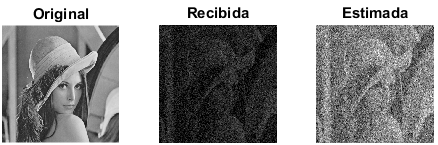
\includegraphics[width=0.9\textwidth]{E1024S20.png}
		\caption{Iteración con $ E = 1024 $ y $ \sigma = 20 $.}
	\end{figure}
	\begin{figure}[H]
		\centering
		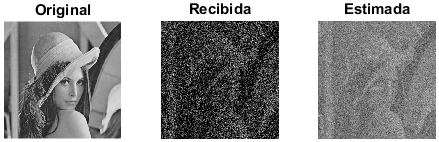
\includegraphics[width=0.9\textwidth]{E1024S50.png}
		\caption{Iteración con $ E = 1024 $ y $ \sigma = 50 $.}
	\end{figure}
	\begin{figure}[H]
		\centering
		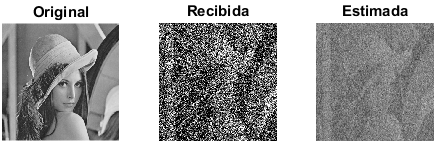
\includegraphics[width=0.9\textwidth]{E1024S100.png}
		\caption{Iteración con $ E = 1024 $ y $ \sigma = 100 $.}
	\end{figure}
		
\end{itemize}

\section{Conclusión}
	Luego de analizar los resultados obtenidos para cada valor de $ E $ y de $ \sigma $, se llegó a las siguientes conclusiones.\par
	Por un lado, queda evidenciado que, para una longitud E fija, a medida que aumenta el desvío estándar en el ruido Gaussiano, la calidad de la imagen recibida disminuye considerablemente, lo que se traduce a su vez, en una imagen estimada que cada vez se aproxima menos a la original.\par
	Por otro lado, si se varía la longitud y se deja fijo el valor de $ \sigma $, se observa que a mayor longitud, mayor calidad de las figuras analizadas, tanto de la recibida como de la estimada.\par
	Se puede concluir que a mayor longitud, el efecto del aumento del desvío estándar es menor que a menor longitud. Por ejemplo, se puede observar que para una longitud de 32, un $ \sigma $ de 50 implica una pérdida total de la imagen original, mientras que con una longitud de 512, para el mismo desvío estándar todavía se puede apreciar cierta similitud entre la imagen estimada y la original, a pesar del alto grado de distorsión.\par
	De la misma manera, a menor valor de $ \sigma $, las diferencias de la calidad de las figuras estimadas para cada valor de longitud son cada vez más despreciables. Se puede observar cómo, para desvío estándar de 0 y 0.1, las figuras correspondientes a cada longitud parecen ser idénticas entre sí.
 
\end{document}
